
%State how sequences are generated.
%State how transition probabilities are generated in the profile chain. State what the profile chain could be used for when collected.

% 3 sections
% Execution assumptions
% algorithmic changes
% producing the profile chain

\section{Execution Environment}

Execution occurs in a real-time partially synchronous environment.
Processes synchronize their clocks and execute steps of the election algorithm at predefined intervals.
Processes with clocks that are not sufficiently synchronized cannot form groups.

\section{Election Algorithm}

A state machine for the election portion of the election algorithm is shown in Figure \ref{fig:statemachine}.
In the normal state, the election algorithm regularly searches for other coordinators to join with.
When another coordinator is identified, all other processes will yield to their future coordinator.
The method of selecting which process becomes the coordinator of the new group differentiates the invitation election algorithm from other approaches.

Coordinators and group members begin in the normal state.
Coordinators identify each other by sending out ``Are You Coordinator'' (AYC) messages.
Receiving processes respond in the positive if they are a coordinator, or the negative if they are not.
In the invitation election algorithm, processes are assigned a priority based on their process ID.
Using the list of coordinators determined with the AYC message, each coordinator determines its relative priority with respect to the other processes that sent the invites.

\begin{figure*}[!t]
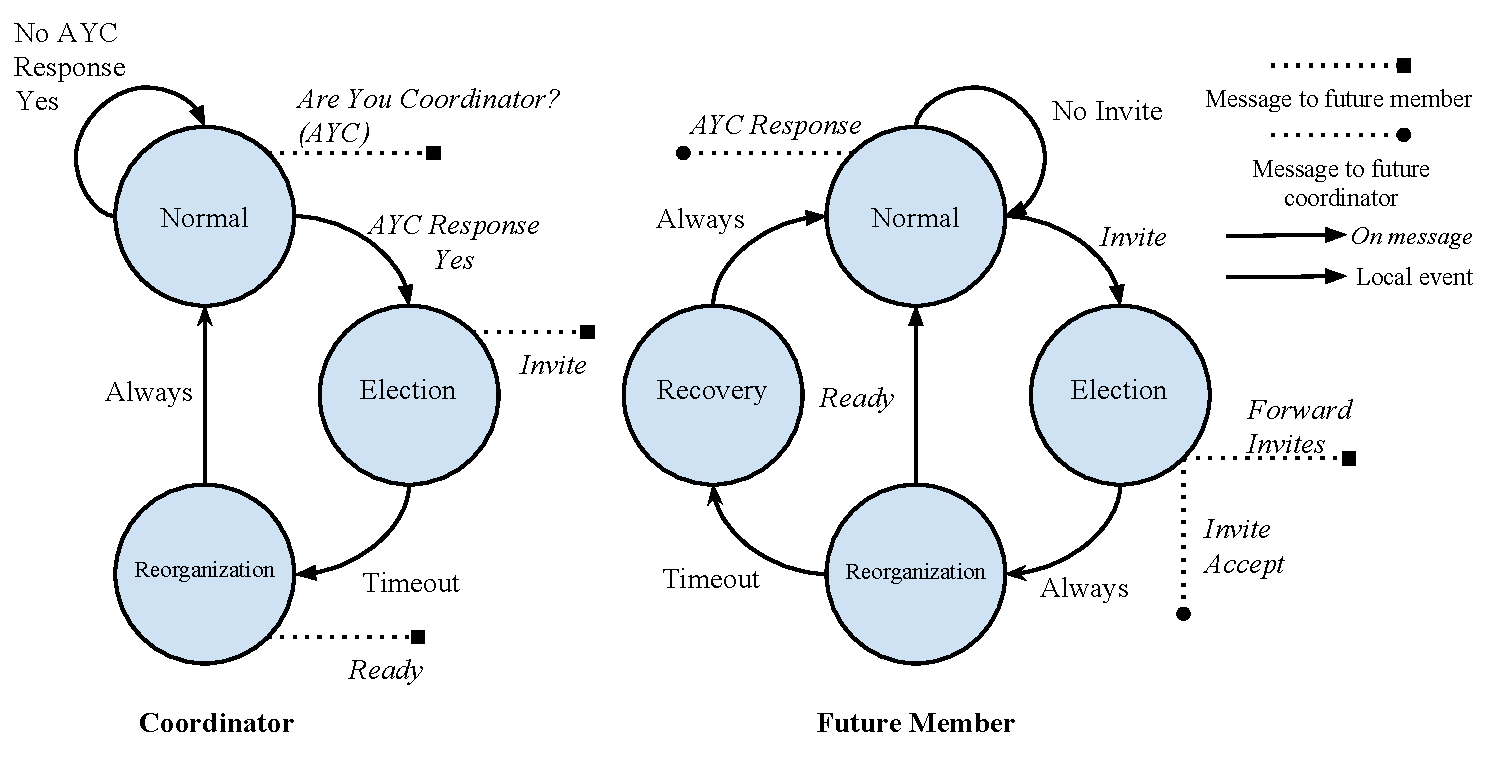
\includegraphics[width=\linewidth]{LeaderElectionStateDiagram.pdf}
\caption{State machine of a leader election. Processes start as coordinators in the ``Normal'' state and search for other coordinators to join with. Processes immediately respond to ``Are You Coordinator'' (AYC) messages they receive}
\label{fig:statemachine}
\end{figure*}

The coordinator with the highest priority is the first to send invites.
When a coordinator sends invites, it switches to the election state.
After a brief delay, if it appears that the highest priority coordinator did not send their invites, the next highest process will send their invites.
A process will only accept an invitation if it is in the normal state.
Coordinators that receive invites will forward the invite to its group members, if it accepts the invite.
Those processes will accept the invite, sending a message to the process that originally sent the invitation.
Once a timeout expires, the coordinator will send a ``Ready'' message with a list of peers to all processes that accepted the invite.
The invited processes have timeouts for when they expect the ``Ready'' message to arrive.
The coordinator, and any process that receives the ``Ready'' message will return to the normal state.
If the ``Ready'' message does not arrive in time for a process, that process will enter the recovery state and reset to a group by itself.

\begin{figure*}[!t]
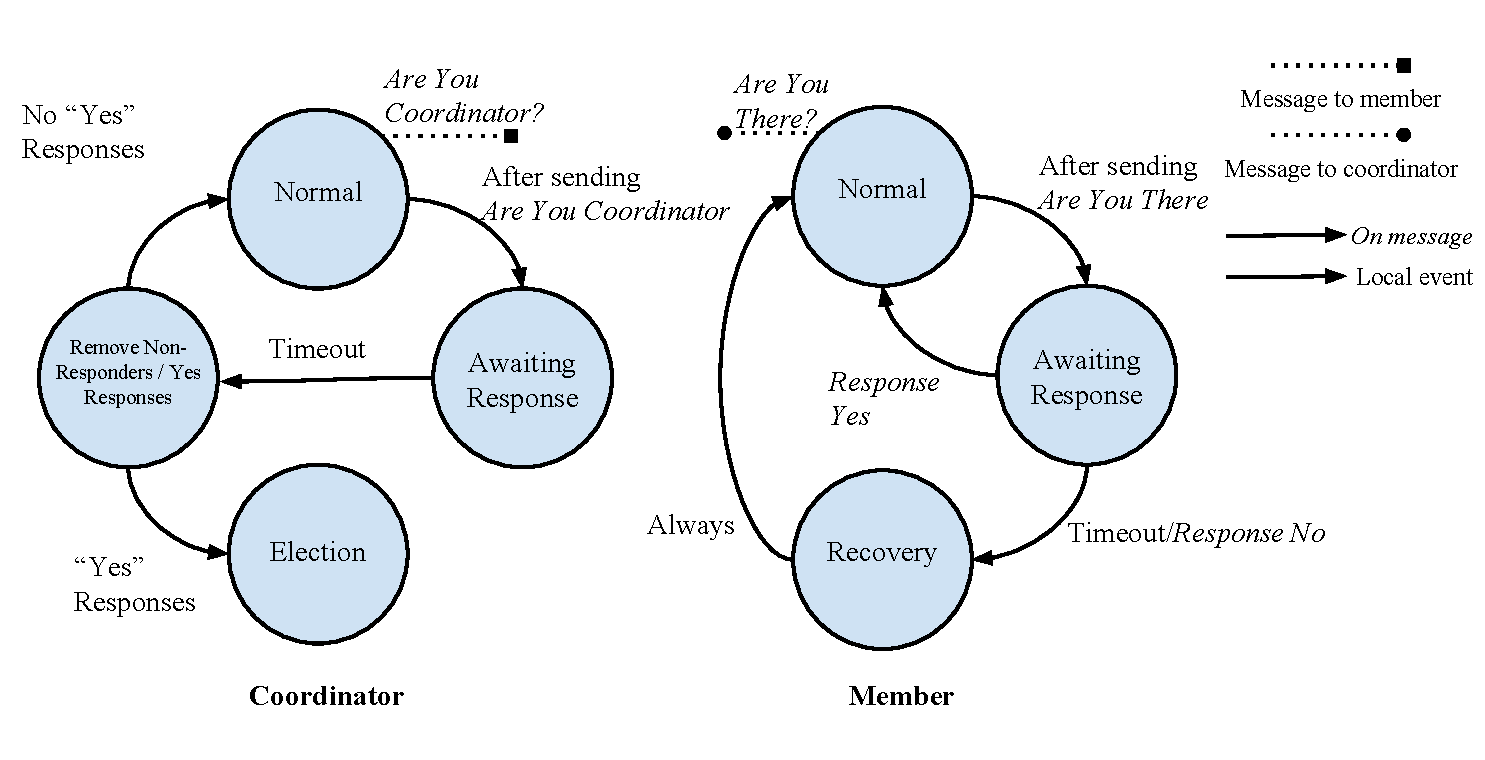
\includegraphics[width=\linewidth]{MaintainStateDiagram.pdf}
\caption{State machine of maintaining a group. The ``Are You Coordinator'' (AYC) messages are the same as those in Figure \ref{fig:statemachine}. AYC and ``Are You There'' (AYT) are periodically sent by processes, and responses to those messages are immediately sent by the receiving process.}
\label{fig:statemachine2}
\end{figure*}


Once a group is formed it must be maintained.
To do this, processes occasionally exchange messages to verify the other is still reachable.
This interaction is shown in Figure \ref{fig:statemachine2}.
Coordinators send ``Are You Coordinator'' messages to members of its group to check if the process has left the group.
If a process does not respond to the AYC message or responds that they are a coordinator, they will be removed from the group. 
Group members send ``Are You There'' messages to the coordinator to verify they haven't been removed from the group, and to ensure the coordinator is still alive.
If the coordinator responds ``no'', or fails to respond, the group member enters the recovery state where it resets to a group by itself.

As part of the DGI's execution, the Group Management module runs before the start of execution for the Load Balancing and State Collection modules.
Each time the algorithm is run the DGI attempts to discover new leaders to merge groups with and verifies the members of its group are still reachable.
